%%%%%%%%%%%%%%%%%%%%%%%
\chapter{システムテストにおけるブラックボックステストの課題}
\section{テストケースの開発方法とテストのレベル}
%−−−-図1を入れる
\begin{figure}[htbp]
  \begin{center}
  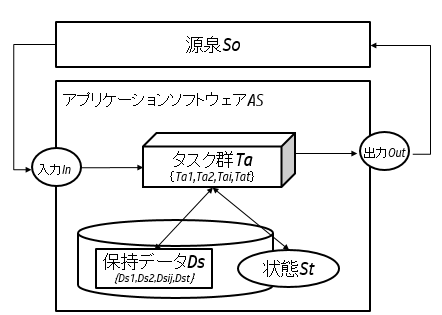
\includegraphics[width=10cm]{./image/fig-1.png}
  \caption{アプリケーションソフトウェアの構成}
  \label{fig:fig-1}
  \end{center}
\end{figure}

\subsection{アプリケーションソフトウェアの構成}
一般的なアプリケーションソフトウェアは,入力$In$に対して,何らかの出力$Out$を返す.
ソフトウェアの機能は,何らかの入力を出力に変換する処理により実現されていると考えられる.
この処理を本論文ではタスクと呼ぶ.
タスクは,該当のテストレベルからみた入力を出力に変換している1処理である.
そのため,タスクの粒度は,後述するテストレベルによって決まる.
ソフトウェアの構成要素であるタスク$Ta$の出力について考えると,$Ta$への入力$In$だけでなく状態$St$と保持データ(データベースや内部メモリに保存されているデータ)$Ds$の影響を受けると考えられる.
例えば,Webアプリケーションにて予約を行うタスクについて考えると,予約が可能か否かを示す状態と,予約オブジェクトの予約状況を示す保持データによって,予約の成否が決まる.
本論文では,対象として図\ref{fig:fig-1}に示すような状態と保持データを持つアプリケーションソフトウェア($AS$)のタスクに対するテストを研究対象にする.
$AS$の構成要素は,タスク群$Ta$と状態$St$と保持データ$Ds$とし,各タスクは外部の源泉$So$からの入力$In$と$So$への出力$Out$があるとする.
タスク群$Ta$は,その要素を$Ta=\{Ta_1,Ta_2,\cdots,Ta_i,\cdots,Ta_t \}$とし, 対応する入出力は$In_i$と$Out_i$とする.

\subsection{テストケースの種類}
テストケースの種類は,ソフトウェアの物理的な構造を基にテスト設計をするホワイトボックステストと,ソフトウェアの仕様を基にテスト設計をするブラックボックステストに大別できる\cite{myers2011art} .

\begin{figure}[htbp]
  \begin{center}
  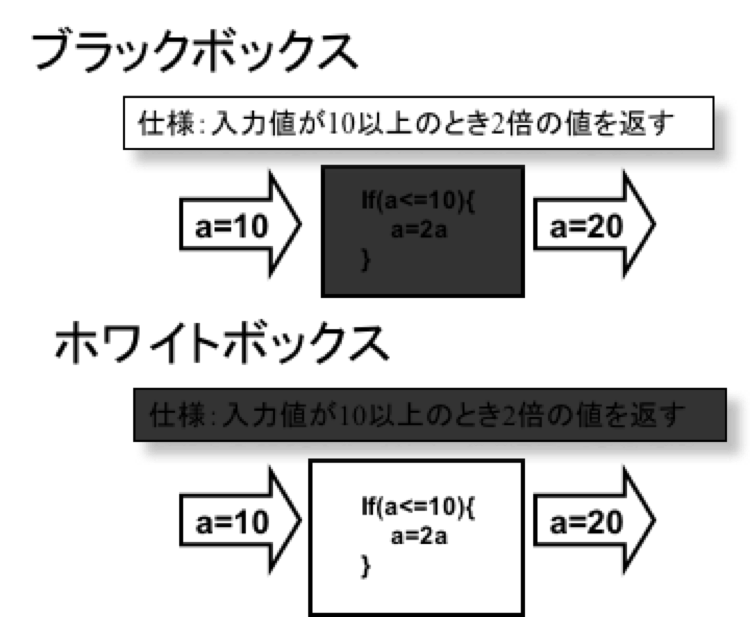
\includegraphics[width=10cm]{./image/BlackboxWhitebox.png}
  \caption{Vモデル1}
  \label{fig:D-2-Fig0}
  \end{center}
\end{figure}



ホワイトボックステストはテスト設計のベースがソースコードのようなテスト対象そのものとなるため,テスト対象プログラムの行を網羅,分岐を網羅といった具合にテストにて網羅すべきアイテムを明確に選択することが容易である.
網羅基準はテスト設計技法として提唱されている\cite{myers2011art,beiz90}.

一方,ブラックボックステストでは,テスト対象そのものではなく,テスト対象の動作条件や振る舞いについて記述した仕様をベースにしてテストケースを開発する.
ブラックボックステストのテスト設計技法の中で、仕様に対する網羅基準は,ホワイトボックステスト同様,数多く提唱されている\cite{myers2011art,beiz90}.

しかし,ブラックボックステストは,テストベースがテスト対象の物理的な構造ではなく論理的なふるまいの記述であるがゆえに,テストを作るための詳細化が複数の解釈で行われることが多い.
結果的にテストケースの重複や抜け漏れを引き起こす可能性も高くなる.

本研究では,設計されるテストケースの種類はブラックボックステストを対象とする.

\subsection{テストレベル}

\begin{figure}[htbp]
  \begin{center}
  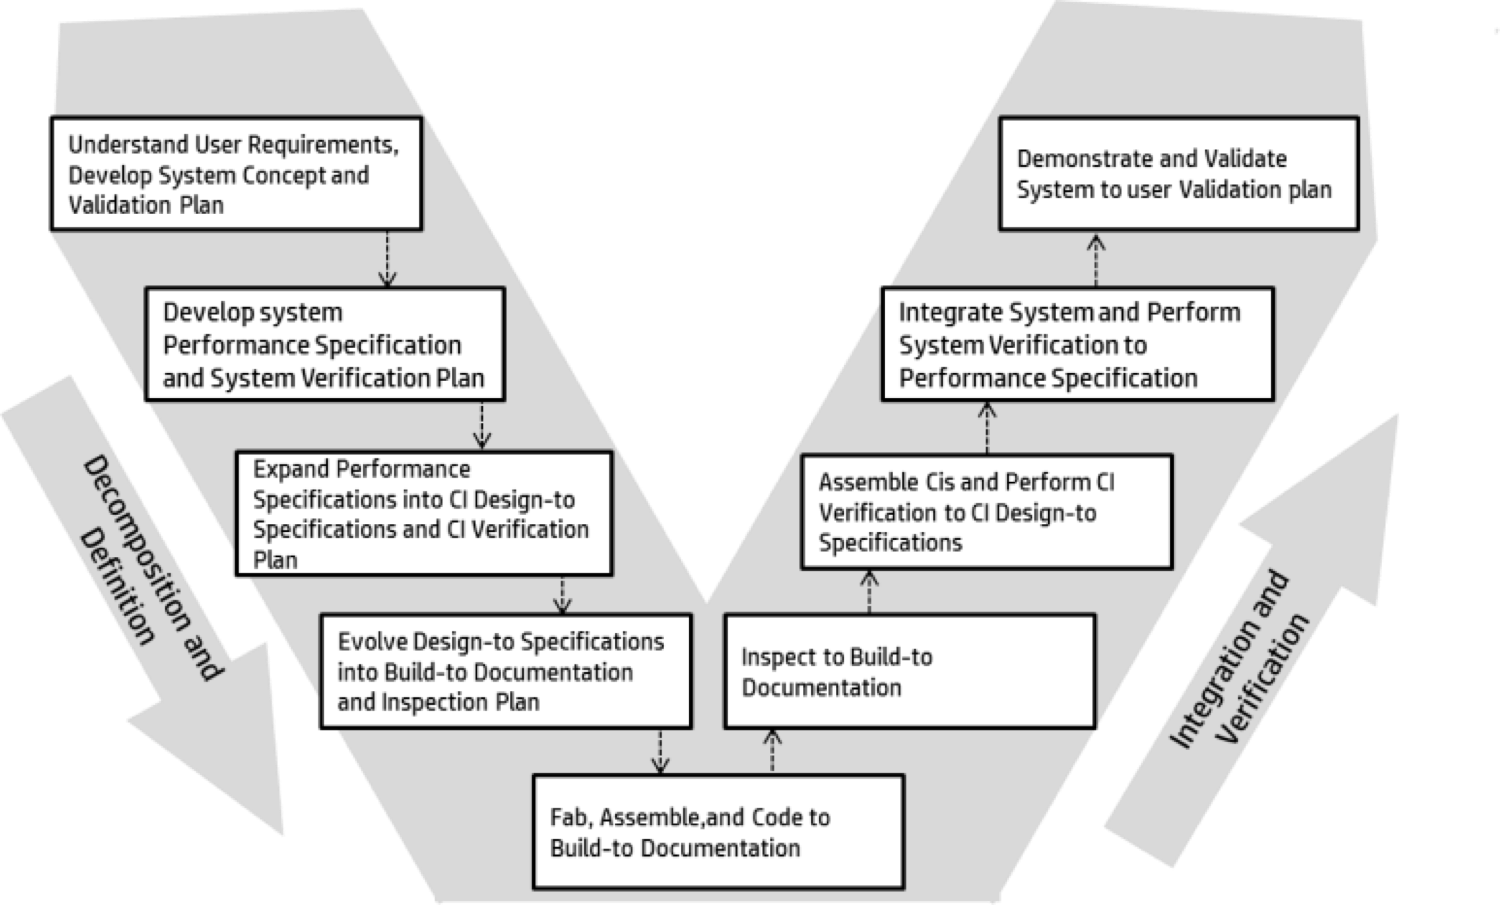
\includegraphics[width=12cm]{./image/D-2-Fig1.png}
  \caption{Vモデル}
  \label{fig:D-2-Fig1}
  \end{center}
\end{figure}
ソフトウェアテストは,開発ライフサイクルの中で複数のテストレベルに分けて行われる.
複数のテストレベルは,図~\ref{fig:D-2-Fig1}で示すVモデルと呼ばれる技術面にフォーカスしたライフサイクルモデルにて表現することができる\cite{forsberg1991}.
各テストレベルはソフトウェア開発の段階的詳細化のレベルと対応している.

テストのプロセスは,Vモデルであらわす各レベルごとに行われる.
本研究は,複数のレベルの中で,図~\ref{fig:D-2-Fig1}の上から2番目の箱となる,「Develop System performance specification and System verification plan」と「Integration system and Perform system verification to performance specificetion」のレベル,つまりシステムレベルのテストで行われるブラックボックステストに焦点を当てている.
システムレベルのテストは,開発した単体のソフトウェアがすべて統合されるため,規模の増大と複雑性の増加の影響を直接的に受けるからである.

\subsection{テスト開発プロセス}
\begin{figure}[htbp]
  \begin{center}
  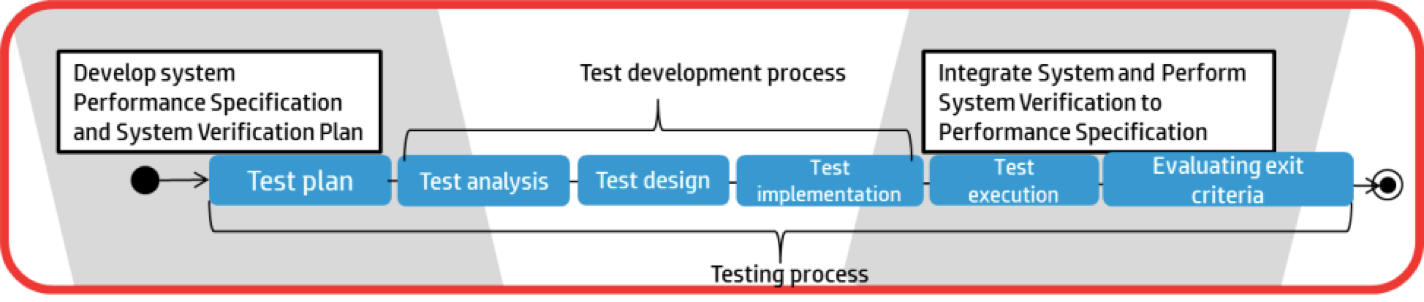
\includegraphics[width=14cm]{./image/D-2-Fig2.png}
  \caption{テスト開発プロセス}
  \label{fig:D-2-Fig2}
  \end{center}
\end{figure}
Vモデルであらわす各レベルにて行われるテストはそれぞれ,開発プロセスと類似したプロセスを持っている\cite{ISTQB}.
テストのプロセスは, 図~\ref{fig:D-2-Fig2}のようにテスト計画がVモデルの左側の活動と並行に行われ,その後時系列にテスト分析,テスト設計,テスト実装が行われた後,Vモデルの右側の活動の中で,テスト実行と終了基準の評価が行われる.
テストのプロセスの中でテスト分析,テスト設計,テスト実装の3つのテストケースを作成するための活動はテスト開発プロセスと呼ばれている\cite{ISTQB}.

本研究では,テスト開発プロセスの中のテスト分析とテスト設計を対象とする.
テスト分析では,テスト対象をテスト設計ができるサイズに詳細化する.
ブラックボックステストでのテストを開発するベースは,対象とするアプリケーションソフトウェアの仕様である.
仕様とは,図~\ref{fig:D-2-Fig1}で示したVモデルの左側の成果物のことである.
各レベルでテスト設計のベースする仕様はテストベースと呼ばれている.
本研究の対象となるテストレベルでは,「Develop System performance specification and System verification plan」のテストベースにて,テスト対象の動作条件や振る舞いについて記述した仕様項目及び仕様項目とそれに該当する事前条件や事前入力の取捨選択をする,整理する.
テスト分析でのアウトプットはテスト条件と呼ばれている.
つまり,テスト条件とは,図~\ref{fig:D-4-Fig1} のように仕様項目と仕様項目に該当する事前条件と事前入力のことを指している.
\begin{figure}[h]
  \begin{center}
  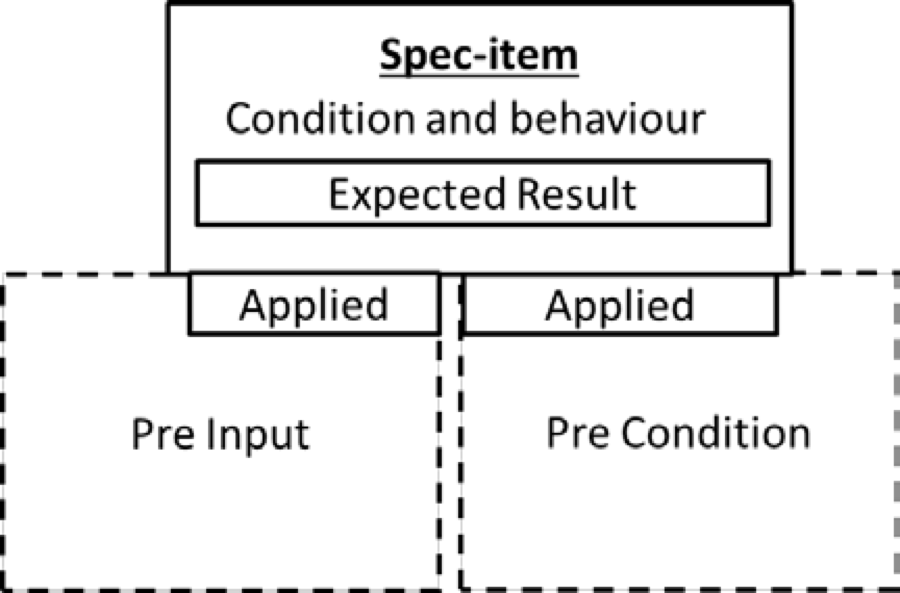
\includegraphics[width=10cm]{./image/D-4-Fig1.png}
  \caption{テスト条件の構成要素}
  \label{fig:D-4-Fig1}
  \end{center}
   \end{figure}

このテスト条件を合理的にある基準で網羅する方法を考える行為がテスト設計であり,そのための技法をテスト設計技法と呼ぶ.
テスト設計のアウトプットはテストケースである.

テストケースは,IEEE610において,特定の目的のために開発されたテスト入力,実行条件,期待結果の3つで構成されると定義している.
また,機能テストは,選択した入力と実行条件のレスポンスとして生成されたアウトプットを確認する,と定義している[ ].
すなわち,タスクに対するテストとは,テスト入力,実行条件,を入力して生成されたアウトプットが期待結果と一致するかを確認することである.
このプロセスを図示すると,図[  ]のようになる.
テスト入力,実行条件には,事前に設定されているものと,実行時点で設定するものがある.
本研究では,おのおのを表[  ]に示すよう定義する.
その上で,事前入力と事前条件をまとめたものをテストパラメータ,イベントと操作をまとめたものをテストアクションと呼ぶこととする.

\section{システムレベルでのブラックボックステストの課題} \label{sec:2-2}
\subsection{テストケースの抜け漏れが起きる課題と関連する先行研究}
テスト分析の活動の出力となるテスト条件は,機能,トランザクション,品質特性,構造的要素といったアプリケーションソフトウェアの側面の総称である.
これらの側面について記述した成果物は仕様とよばれる.
テスト分析では,テスト対象をテスト設計ができるサイズに詳細化する際にこれらの側面が記述されている仕様に着目して詳細化を行う.
その際は,テスト対象の詳細化をするときの起点や中間分類が人によって異なってバラバラになってしまわなように各側面の関係を整理する必要がある.
しかし,テスト分析におけるテスト条件群の整理方法は,研究や実務においても,経験則や個人の考え方に基づいている.
一般的には,テストベースを大項目,中項目,小項目と詳細化していくことが多い.
この方法は,詳細化する際の各分類項目に当てはめるアプリケーションソフトウェアの側面に明確なルールが定義されていないため,個人毎の何かしらの考え方で詳細化するための分類を決めていくことになる.
そのため,複数人で作業を行うと分類にばらつきが発生し,同じテスト条件が複数の階層に現れてしまったり,同じ意味のテスト条件が別の名称で選択されるといった混乱が起きてしまう.
混乱が起きている例を表~\ref{tab:analysissample}に示す.
% Table generated by Excel2LaTeX from sheet '論文挿絵'
\begin{table}[htbp]
  \centering
  \caption{Add caption}
    \begin{tabular}{|l|l|l|l|l|p{9.335em}|}
    \hline
    大項目   & 中項目   & 小項目   & 細目    & 補足項目  & テスト条件 \bigstrut\\
    \hline
    印刷    & 設定    & 印刷部数  & ー     & ー     & 100部印刷した場合 \bigstrut\\
    \hline
    設定    & プリント設定 & 一般    & 異常系   & エラーメッセージ & 「印刷部数が99部を超えました」と表示されること \bigstrut\\
    \hline
    \end{tabular}%
  \label{tab:analysissample}%
\end{table}%
表~\ref{tab:analysissample}の例には以下のような問題がある.
\begin{enumerate}
\item 設定というカテゴリが大項目に出ている場合と中項目に出ている場合が混在している.
\item 階層数も一定でないため,各階層がどのような意味を持つものかがばらついている.
\item 上段は,期待結果が書かれていない.
\item 上段と下段は同じテスト条件について書かれている.
\end{enumerate}
テスト開発の最初の活動であるテスト分析にて特定するテスト条件にこのような問題があると,その後の活動で作られるテストケースの抜け漏れ,重複に影響を及ぼす.
ISTQBでは,テスト分析は「…テスト分析の期間中,何をテストするか決定するため,すなわち,テスト条件を決めるために,テストのベースとなるドキュメントを分析する [ ] 」と説明されている.
ISTQBでは,この説明のとおり,テスト分析を実行するための要求事項や必要性は述べているけれども,テストベースを分析していくためのアプローチは定義されていない.
これは,Ostrand [ ], Grindal [ ]などのテスト開発に関する先行研究でも同様である.
更に言うと,G.J.MyersやB.Beizerといった先行研究の多くは,テスト分析にてテスト条件が特定された後のテスト設計で行われるテストパラメータの設計に焦点を当てている.
そのため,テスト条件は,すでに全て準備されたと言う前提になっている.
テスト分析手法に関する研究は,Nishi\cite{nishi2012based}, Akiyama\cite{Akiyama2014}, Yumoto\cite{yumoto2013test}がある.
それらの研究はテスト分析手法の論理に着目をしているけれども,複数の人数でテスト分析を行う際のテスト条件の重複と欠落について,手法を適用すると実際はどの程度効果的であるかについては,大きく着目していない.
Eldh は,Understanding Instructionの不足によるテストケースの品質低下について調査をしており,複数の解釈による間違いが起きることを報告している [10] .
テスト分析のルールが一貫性を持っていないことは同様の問題を引き起こす.また,ルールに一貫性がないことはテストの再利用を困難にする.

\subsection{テストケース数が増えてしまう課題と関連する先行研究}
テストケース数の増加は,単一機能のテストより機能間の統合において問題となる.
この場合のテストケース数は,単一の機能や制御構造の和で求めるのではなく,積となるためである.
それに加え,このテストでは,状態遷移に伴う時系列の組合せのテストも求められることから,テストケース数の爆発問題が生じる.しかし,必要なテストケースの抽出方法とその網羅性に関する研究は多々あるが,多くは機能や制御構造を基にした方法である.\cite{myers2011art}

状態遷移間の組合せについては,N スイッチカバレージに従ってテストケースを抽出する方法がある. \cite{beiz90}
N スイッチカバレージとは,状態の遷移をパスとし,N+1 個の遷移パスを網羅する基準に従て組合せテストケースを作成する.
N=0 では遷移パスの組合せをテストできないため N=1,すなわち S1 網羅基準(1 スイッチカバレージ)が必要とされている.しかし,S1 網羅基準を満たすテストケース数は, 2つの状態遷移間における遷移数の積となり,膨大なテスト工数を必要とする課題になる.

\section{テストカテゴリベースドテスト}
本研究では,テストカテゴリベースドテストという分析手法を利用した検証実験を行い,テスト分析の課題の調査を行う\cite{yumoto2013test}.
この分析手法を採用する理由は,3つある.
1つは,前述するテスト分析の課題を解決するために自身で提案し,現場にて適用している手法であるためである.
2つめは,検証実験のための題材となる仕様書,模範解答が揃っており,それらの題材を使って実験を行った研究結果があるためである.
3つめは,本研究で合理的にテストケースの抽出を行う手法を提案する基の考え方として,テストカテゴリベースドテストを基にしていることである.

本節では,テストカテゴリベースドテストの概要を説明する.
このテスト分析手法のアプローチでは,テスト条件群を,テスト対象のサブセットとなるフィーチャセットに属するタスクとテストケースの構造をベースに階層化することで,テスト条件と言う用語の持つ曖昧さを排除している.
タスクとは,前述した通り,アプリケーションソフトウェアにて何らかの入力を出力に変換する処理のことである.
また,階層の要素としてテストカテゴリという,テスト対象の知識とフォールトの知識使って定義した分類を構造に追加した.
テストカテゴリをテスト分析のガイドとして使い,抜け漏れや重複の少ないテスト条件の選択を可能にする.

\subsection{テスト条件群の構造}
前述した通り,テスト条件とは,機能,トランザクション,品質特性,構造的要素といったアプリケーションソフトウェアの側面の総称である.
通常,これらはアプリケーションソフトウェアの仕様として記載されるものである.
ブラックボックステストにおけるテスト条件群の要素は,図~\ref{fig:D-4-Fig4}に示した構造で整理できる.

\begin{figure}[htbp]
  \begin{center}
  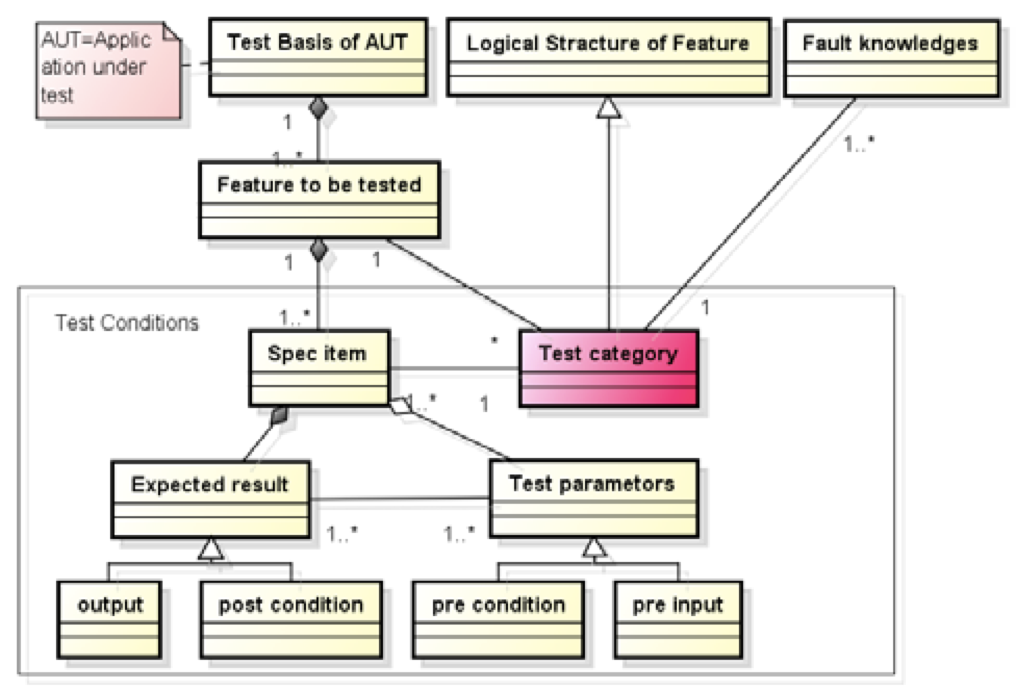
\includegraphics[width=8cm]{./image/D-4-Fig4.png}
  \caption{テスト条件の構造}
  \label{fig:D-4-Fig4}
  \end{center}
   \end{figure}


テストベースは,テストケースを抽出する基になる文書のことであり,開発時に作成する要件や設計内容が書かれた文書が該当する.
テストベースにはテスト対象フィーチャを実現するタスクを明確に定義する仕様項目が1つ以上記述されている.
フィーチャは,利用者が観察可能なソフトウェアシステムのサブセットであり,利用者とテスト対象のインターフェースとなる[ ].
ブラックボックステストは,外部観察によるテスト設計の方法であるため,テスト条件をフィーチャから選択することが必要になる.
テスト対象から選択したフィーチャはテスト対象フィーチャと呼ばれている[ ].

仕様項目とは,テスト対象フィーチャに属するタスクの要件を綿密に定義し文書化したものである.
タスクの要件とは,テスト対象フィーチャの振る舞いのひとつであり,たとえば「ボリュームは1 から10 の間で設定できる.1 は消音であり,10は100dbsになる」が該当する.
この記述が仕様項目である.
テスト分析では,テストすべき仕様項目を選択していく.
その仕様項目の内容をテストケースの構成と同じように期待結果とテストパラメータに分類し,整理する.
テストパラメータとは,テストケースの構成要素のひとつで,事前入力と事前条件を汎化したものである[9].
このような分類,整理によって,明確なルールにそったテスト分析が可能になる.

\subsection{論理的機能構造}

\begin{figure}[htbp]
  \begin{center}
	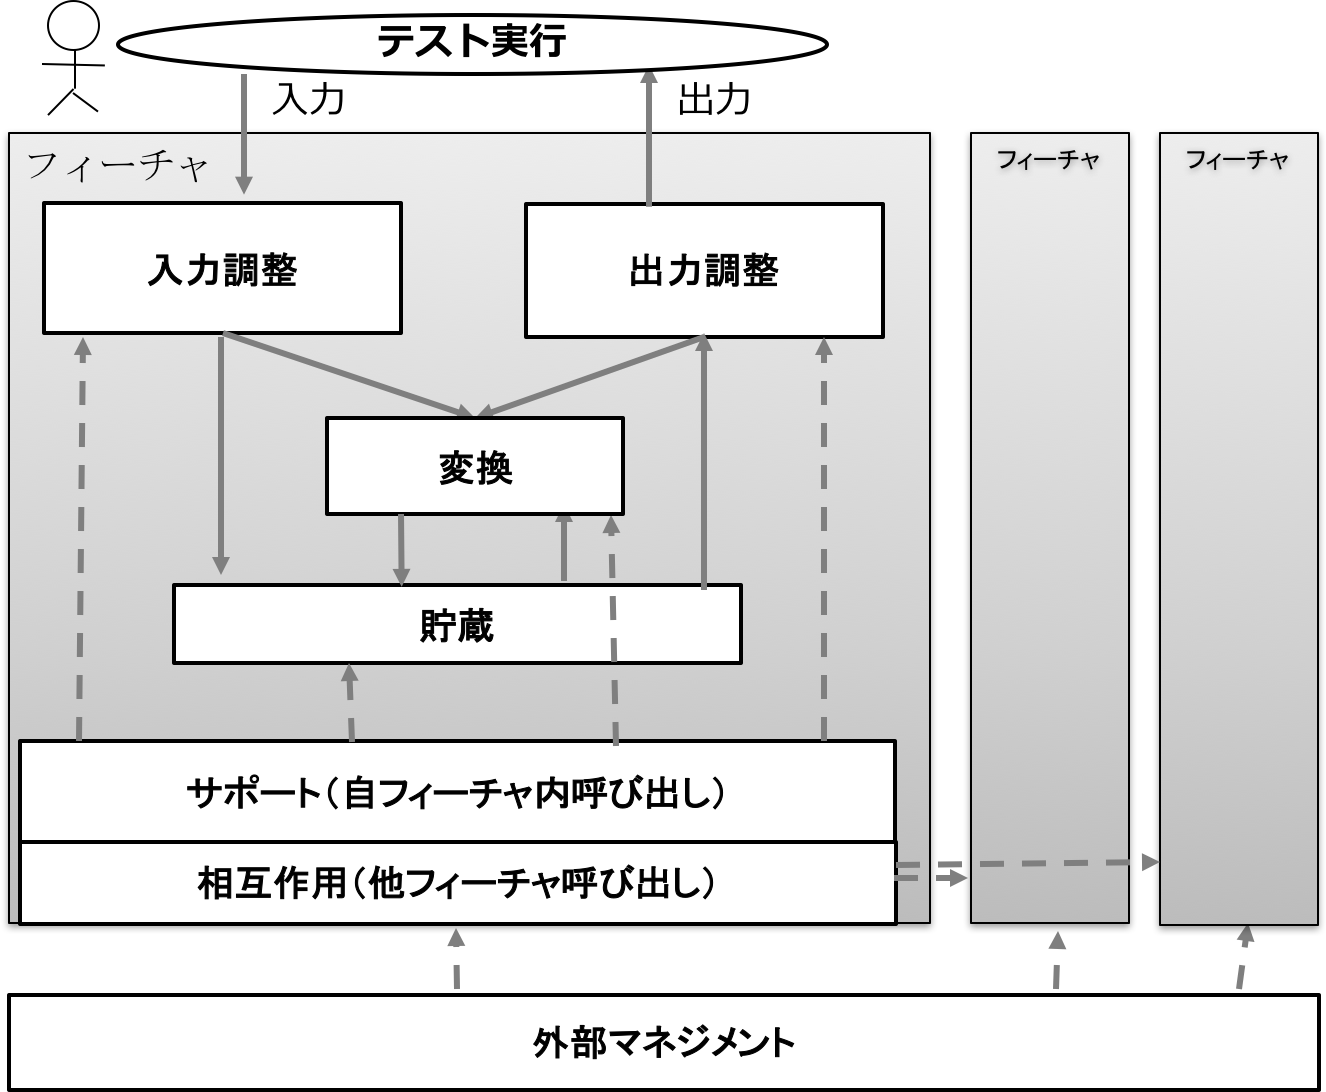
\includegraphics[width=10cm]{./image/D-3-Fig3.png}
	\caption{MECEにフィーチャからテスト条件を識別する方法}
	\label{fig:D-3-Fig3}
  \end{center}
\end{figure}

ブラックボックステストの場合,テスト対象の内部構造を完全に知ることはできなく,テスト実行は入力と出力だけが頼りになる.
大村は「…人工のシステムとは,インプットを変換し付加価値を与えアウトプットする変換装置であるため,論理的には,必ず図「 」のような構造を持つ[  ]」と主張している.
提案しているテスト分析手法は,同様のコンセプトを利用している.
つまり,テスト対象のフィーチャ[ ] は同様の論理構造を持つ人工システムだと考えている.
この論理構造は,図「 」のようにフィーチャをMECE(互いに相容れなくて完全に徹底的)\cite{ethan1999mckinsey}な方法でテストをするために利用できる.
図「 」に示す各箱は,テスト対象の内部構造を推定し,テストが必要なタスクを特定する有用なモデルとして利用できる.
そして,タスクに関する記述がされている仕様項目がテスト条件となる.

テスト分析をしていく際に論理的機能構造を使って内部構造を推定してタスクを特定していく方法を導入すると,テストに必要なテスト条件の特定が容易になるという仮説を立てている.
現状,次に示す課題はテスト条件の特定を困難にしている.

\begin{enumerate}
\item 明白に必要だと思われる仕様の一部分が記述されていない.
\item 機能間の組み合わせでどのように振舞うかといった仕様は,ドキュメント中の該当する単一のセクションには完全に記載し切れていない.
\end{enumerate}

\subsection{テストカテゴリ}
論理的機能構造は抽象的な概念であるため,テスト分析をするそれぞれの技術者の間にて解釈の違いが生じる可能性がある.
テスト条件を決定する際に,その解釈に一貫性を持たせるため、論理的機能構造の箱に対してテスト対象で使われる用語を使った名前付けをする.
そのようなテスト対象に特化して付けた論理的機能構造の各箱の名前をテストカテゴリと呼ぶ.
テストカテゴリはテスト条件を特定するための有用なガイドである.
特定したテスト条件にはフィーチャの仕様項目,期待結果,テストパラメータが含まれている.
決定したテストカテゴリに対する合意形成は,最も重要なことになる.
各メンバーが各テストカテゴリの意味を明確に理解していることを確認するために,メンバー間での各テストカテゴリに分類したテストにて発見する可能性のある欠陥および故障を,例を挙げてディスカッションすることを必須にしている.

\begin{table}[htbp]
  \centering
  \caption{テストカテゴリ一覧の例}
    \begin{tabular}{|p{6em}|p{8.07em}|p{14.645em}|}
    \hline
    \textbf{論理的構造} & \textbf{テストカテゴリ} & \textbf{意味づけ(想定する欠陥)} \bigstrut\\
    \hline
    \multirow{2}[4]{*}{\textbf{入力調整}} & \textbf{画面入力} & \textbf{入力チェック,入力画面の制御} \bigstrut\\
\cline{2-3}    \multicolumn{1}{|l|}{} & \textbf{ボタン操作} & \textbf{画面遷移のルール,処理起動} \bigstrut\\
    \hline
    \textbf{出力調整} & \textbf{表示} & \textbf{処理結果の表示,出力数の制御} \bigstrut\\
    \hline
    \multicolumn{1}{|r|}{} & \textbf{帳票出力} & \textbf{印刷内容,印刷フォーマット} \bigstrut\\
    \hline
    \textbf{変換} & \textbf{計算} & \textbf{料金計算} \bigstrut\\
    \hline
    \multirow{2}[4]{*}{\textbf{貯蔵}} & \textbf{検索} & \textbf{検索条件の組み合わせ,検索結果} \bigstrut\\
\cline{2-3}    \multicolumn{1}{|l|}{} & \textbf{登録/更新/削除} & \textbf{DB処理} \bigstrut\\
    \hline
    \textbf{相互作用} & \textbf{反映} & \textbf{DB処理結果の他機能への反映} \bigstrut\\
    \hline
    \textbf{サポート} & \textbf{エラー処理} & \textbf{エラー復旧処理} \bigstrut\\
    \hline
    \end{tabular}%
  \label{tbl:D-4-tbl1}%
\end{table}


テストカテゴリに関するディスカッションの結果は表~\ref{tbl:D-3-tbl1}で示した表にまとめる.

それによりテスト開発プロセス活動にかかわるメンバーは認められたテストカテゴリに対して合意形成をすることができる.
合意形成のねらいは次のとおりである.

\begin{enumerate}
\item テスト開発にかかわるテスト担当がAUT に関して同様の理解に達することができる.
\item テスト担当間のテスト条件の解釈のぶれを最小限にとどめることができる.
\end{enumerate}


\subsection{実施手順とドキュメントフォーマット}
構造化したテスト条件群を順番に導くために,テスト分析の活動を図~\ref{fig:D-4-Fig3}のような作業ステップに分割し,各ステップでのインプットとアウトプットを定義する.


\begin{figure}[htbp]
  \begin{center}
  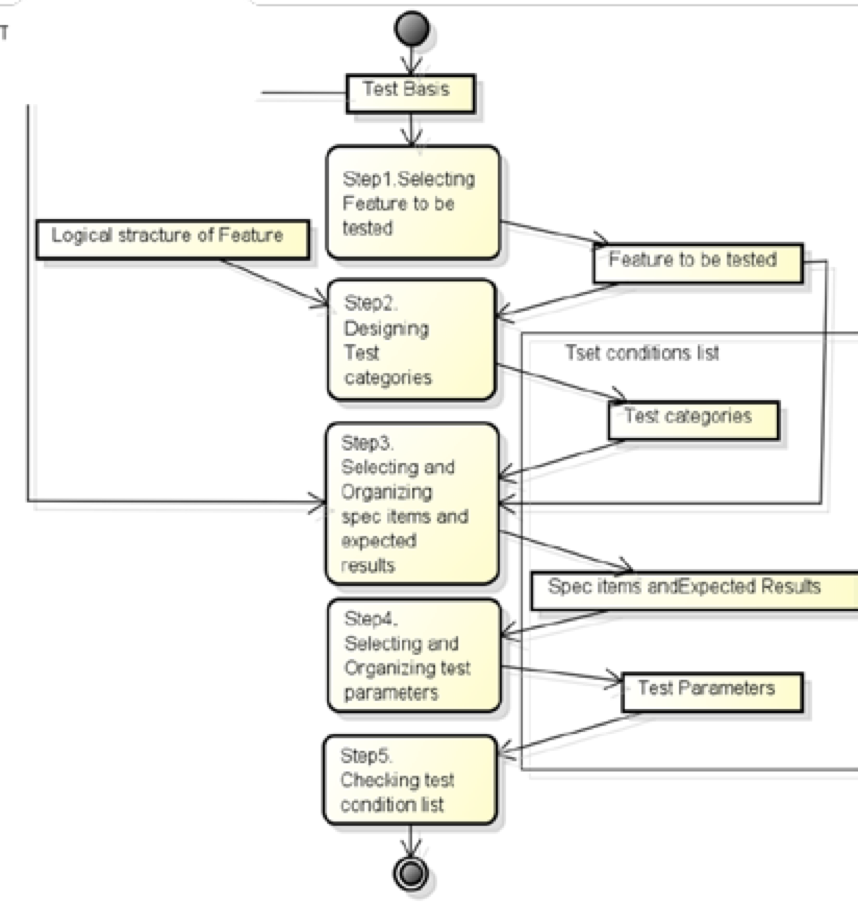
\includegraphics[width=12cm]{./image/D-4-Fig3.png}
  \caption{テスト分析の実行ステップ}
  \label{fig:D-4-Fig3}
  \end{center}
   \end{figure}


以降に各作業ステップについて説明をする.

\begin{description}
\item[Step1] テスト対象のフィーチャを選択

テストベースからテスト対象のサブセットとなるフィーチャを特定する.フライト予約をするソフトウェアで例えた場合,フライト予約(搭乗したい飛行機の条件を照合し,予約を成立させる一連の機能群)がテスト対象フィーチャとなる.

\item[Step2] テストカテゴリの設計

テストカテゴリを設計する方法は,階層ホログラフィックモデリング法(HHM法)におけるサブトピックの設定方法と類似している\cite{HHM2002}.
HHM法でいうところのメイントピックにテスト対象フィーチャを置く.
メイントピックを構成するサブトピックとして論理的構造毎にテスト対象フィーチャの動作条件や振る舞いを列挙する.
列挙する際はどのようなフォールトが起きることが考えられるかを検討材料にして列挙する.
選択したテスト対象フィーチャ全部に対してサブトピックを列挙した後に,サブトピック全体を眺めて,象徴する名称を付与し,それをテストカテゴリにする.
テストカテゴリは,メンバ間で内容を説明し,意味づけ(フォールトの言い換え)を共有することで,解釈のぶれを防ぐ.


\item[Step3] テストカテゴリを使い仕様項目と期待結果を選択,整理する.

テストカテゴリでフィーチャの内部構造を推定し,実現するタスクを特定する.
テストベースからそのタスクの仕様項目と期待結果の記述を抽出する.


\item[Step4] テストパラメータを選択し,整理する.

選択した仕様項目と期待結果からテストパラメータを選択する.テストパラメータは選択した仕様項目と期待結果にヒントとなることが書かれているため,それを手がかりにテストベースを分析して選択する.

\end{description}



% Table generated by Excel2LaTeX from sheet 'Sheet2'
\begin{table}[htbp]
  \centering
  \caption{テスト条件一覧の例}
    \begin{tabular}{|c|p{6em}|p{6em}|p{6em}|p{7.145em}|}
    \hline
    \multicolumn{1}{|p{8.855em}|}{\textbf{テスト対象フィーチャ}} & \textbf{テストカテゴリ} & \textbf{仕様項目} & \textbf{期待結果} & \textbf{テストパラメータ} \bigstrut \\
    \hline
    \multicolumn{1}{|c|}{\multirow{4}[8]{*}{TF-a}} & TC-a  & SI-a  & ER-a  & TP1,TP2 \bigstrut\\
\cline{2-5}          & \multicolumn{1}{l|}{} & SI-b  & ER-b-1 & TP1,TP3,TP4 \bigstrut\\
\cline{2-5}          & \multicolumn{1}{l|}{} & \multicolumn{1}{l|}{} & ER-b-2 & TP1,TP4 \bigstrut\\
\cline{2-5}          & TC-b  & SI-c  & ER-c  & TP5,TP6,TP7 \bigstrut\\
    \hline
    \multicolumn{1}{|c|}{\multirow{2}[4]{*}{TF-b}} & TC-a  & SI-d  & ER-d  & TP9,TP10 \bigstrut\\
\cline{2-5}          & TC-b  & N/A   & N/A   & N/A \bigstrut\\
    \hline
    \end{tabular}%
  \label{tbl:D-3-tbl3}%
\end{table}%

テストベースからテスト条件を特定する際は,その結果を表~\ref{tbl:D-3-tbl3}に示すテスト条件リストにまとめる.

% Table
\begin{table}[t]
\caption{テスト条件一覧の例 未作成}
\label{tbl:D-3-tbl2}
\begin{center}
\begin{tabular}{r|r|r|r}
機能構造&テストカテゴリ&例&故障の例\\
\hline
\hline
変換&計算&料金の計算&計算ミス\\
\hline
入力調整&UIからの入力&画面からの入力&エラー\\
\hline
相互作用&反映&画面からの入力&エラー\\
    \hline
\end{tabular}%
%\halflineskip
\end{center}
\end{table}



各テスト対象フィーチャには同じテストカテゴリのセットを列挙する.
そして,各テストカテゴリに対応する仕様項目と期待結果を列挙する.
テスト対象フィーチャによってはテストカテゴリに対応する仕様項目が無い場合もあり,その場合はテストカテゴリの中に列挙されるものが何も無いのでN/A と記載する.




仕様項目によっては,条件によって期待結果が複数になることがあるため,その際は,リストには仕様項目に対して複数の期待結果を記載する.
テスト条件リストの作成を通じて,各仕様項目と期待結果のセットに要求されるテストパラメータの組み合わせが特定できるようになる.テストパラメータはテスト設計プロセスの中で同値クラスと組み合わせを設計する.
セクションI にて示したとおり,テストパラメータを設計するための手法や技法に焦点を当てた研究は数多くなされている.


多くのテスト開発に従事するテスト担当者が上記のステップに従うと,その全てのテスト担当者は,同じルールに沿って各自の仕事を実行できる.
結果として,開発されたテスト条件のまとまりは,より包括的で,重複が含まれない.
これは総合的に見て高いテストカバレッジを確かにし,高品質のテストを提供することにつながる.
これは本手法の主たる効果となる.
更に,この手順には3つの効果がある.

\begin{enumerate}
\item この手順は,本手法で提案しているテスト条件の構造をベースにしている [6]. テストベース内の要素は,仕様項目,期待結果,テストパラメータに分類できる.この手順を通して,各要素は1つずつ順番に特定,選択する. テスト分析にて同じロジックと手順で作成し,同じカテゴリに分類できた各メンバーの最終結果の可読性が向上する.
\item テストカテゴリに対する合意形成によって,チームメンバは仕様項目の特定と選択が容易になる.
\item 本手法は体系化され,標準化され,進めていくのか用意になるため, テスト担当者がテスト分析を繰り返すことができるようになる.
\end{enumerate}

\subsubsection{テストカテゴリ活用有無によるテスト条件導出結果の比較}

テスト設計に関するワークショップを開催し,2チームに分かれてテスト分析の作業ステップ3「テストカテゴリを使った仕様項目と期待結果の選択」の演習を行った.
ひとつのチームは,テストカテゴリを使わずに仕様項目,期待結果,テストパラメータを列挙してもらい,もうひとつのチームは,テストカテゴリを使って仕様項目,期待結果,テストパラメータを列挙してもらった.題材として音楽再生機器を選定した.出席者は全てこの機器のテストに関わった経験があり,製品知識はある.テスト対象フィーチャは,音楽再生機器のボリュームコントロール機能を選定した.

これまでの実験では,同一組織内で本分析手法を導入したグループと導入していないグループでのテスト条件の選択数を比較する実験結果を行なった.
グループの回答を実験データを使った理由は,この手法の効果が複数の人員でテスト分析をしたときのばらつきからくる欠損や重複を防ぐことを狙っているためである.

この実験にて,分析手法を導入したグループが, 導入していないグループよりも抜け漏れが少なく重複も少ない結果となった.

一貫性のあるルールを適用することでテストケース作成に必要な仕様項目の特定の際に抜け漏れが少なくなることを確認している.しかしながら,今までの研究にて提案した手法は,テストベースの分析に論理的機能構造をガイドとして使用することを明示しているだけであり,具体的な分析手順について定義できていない.そのため,実験の際に被験者に対して,テスト分析にて仕様項目の選択を網羅的に行う具体的な方法を明確に提示できていない.
